This section focuses on problems of offline solving simultaneous-move games. 
The baseline algorithm for solving simultaneous-move games is backward induction~(Section~\ref{sec:algs:bi}).
Therefore, we start our description of the algorithms focusing on algorithms based on the backward induction, then we introduce algorithms based on no-regret learning and Monte Carlo sampling.
After formally describing the backward induction we present a modification that exploits quick calculation of upper and lower bounds in a simultaneous-move game~(Section~\ref{sec:algs:biab}).
Then, we further improve the algorithm by speeding up the calculation of NE in stage games, exploiting the iterative framework known as the double-oracle algorithm~(Seciton~\ref{sec:algs:doab}).
\bbosansky{CFR/MCTS introduction}

\subsection{Backward Induction}\label{sec:algs:bi}
Standard backward induction algorithm is based on the depth-first search that in each state of the game evaluates all successors, creates matrix game for the current state, solves the matrix game, and propagates back the value of the matrix game. The pseudocode of the algorithm is depicted in Algorithm~\ref{alg:backwardinduction}. When there is a chance node succeeding the current state $s$, the algorithm directly evaluates all successors of this chance node calculating an expected utility: the value of each subgame rooted in node $s'$ calculated by recursive call is weighted by the probability of the stochastic transition $\Delta_{\cT(s,r,c)}$~(line~\ref{alg:bi:recursive}).

\begin{algorithm2e}[t]
\small
\SetKwInOut{Input}{input}\SetKwInOut{Output}{output}
\Input{$s$ -- current matrix game; $i$ -- searching player}
\If{$s \in \cZ$} {\Return $u_i(s)$} \label{alg:bi:stop1}
\For{$r \in \cA_1(s)$}{
	\For{$c \in \cA_2(s)$} {
	$A_{rc} \leftarrow \sum_{s' \in S \;:\; \Delta_{\cT(s,r,c)}(s') > 0} \Delta_{\cT(s,r,c)}(s')\cdot \textrm{BI}(s',i)$ \label{alg:bi:recursive}\;	
	}
}
$v_s \leftarrow$ solve matrix game $A$\;
\Return $v_s$ \label{alg:bi:stop2}
\caption{Backward Induction.}\label{alg:backwardinduction}
\end{algorithm2e}

Once the algorithm evaluates the value of each possible subgame following the current state $s$, then the matrix game $A$ is complete and the algorithm solves the matrix game $A$ using standard linear program (LP) for solving normal-form games:
\begin{eqnarray}
\max & v_s & \\
\textrm{s.t.} & \sum_{a_i \in \cA_{i}}A_{a_i,a_{-i}} \cdot \delta^{s}_i(a_i) \geq v_s & \forall a_{-i} \in \cA_{-i}\\
& \sum_{a_{i} \in \cA_{i}} \delta^{s}_{i}(a_{i}) = 1 \\
& \delta^{s}_{i}(a_{i}) \geq 0 & \forall a_{i} \in \cA_{i} 
\end{eqnarray}
Using the linear programming, the algorithm computes the value of the matrix game, which is propagated to the predecessor~(line~\ref{alg:bi:stop2}). 
If the algorithm evaluates a terminal state, it directly returns the utility value of the state~(line~\ref{alg:bi:stop1}).

Solving the linear programs is the main computational bottleneck of the backward induction algorithm. Therefore, in the following algorithms, we try to avoid this step of the computation even for the price of multiple traversal of the game tree.

\subsection{Backward Induction with Serialized Alpha-Beta Bounds}\label{sec:algs:biab}
Backward induction algorithm can be easily enhanced by using bounds on the value of sub-games. 
These bounds can be calculated very quickly by using a transformation of a simultaneous-move game into a perfect information extensive-form game.
Consider a matrix game representing a simultaneous choice of both players.
This matrix can be serialized by discarding the notion of information sets; hence, letting one player to play first following by the play of the second player. 
The crucial difference between a serialized and a simultaneous-move matrix game is that the second player to move has an advantage of knowing what action has been played in a serialized game.
Therefore, the value of a serialized game where player $i$ is second to move is an upper bound on the value of the matrix game. 

\begin{figure}
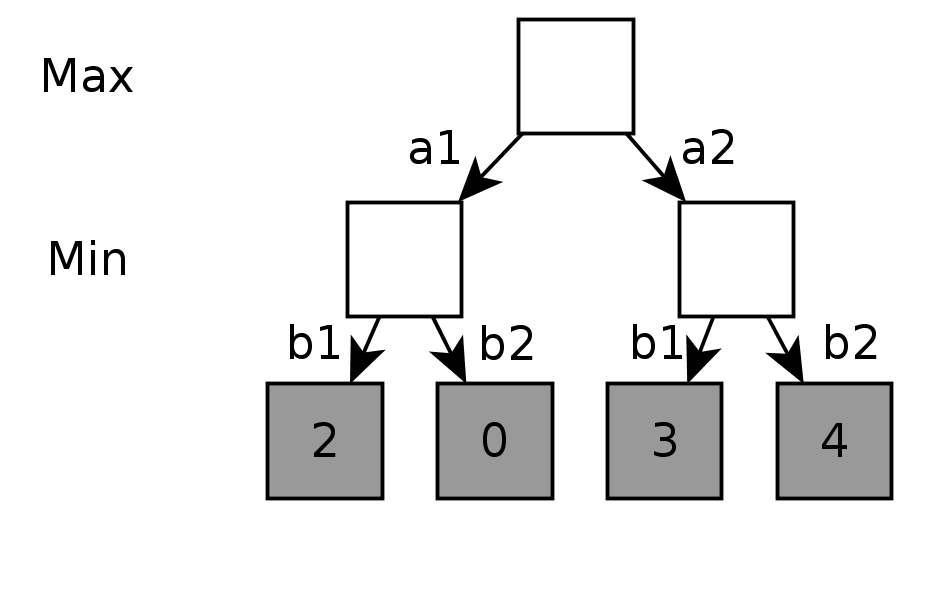
\includegraphics[width=0.45\textwidth]{figures/serialization1-1.png}
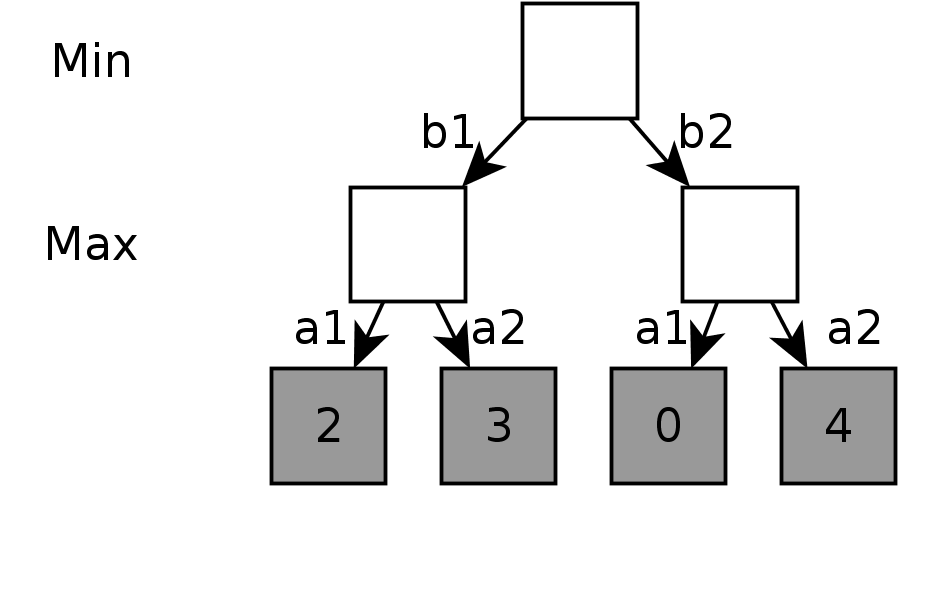
\includegraphics[width=0.45\textwidth]{figures/serialization1-2.png}
\caption{Different serialization of a simultaneous move game.}\label{fig:serialization}
\end{figure}

An example of this serialization is depicted in Figure~\ref{fig:serialization} with the utility value in the leaves depicted only for the first player. 
If this player moves first (the left subfigure), then the value of this serialized game is the lower bound of the value of the game; if this player moves second (the right subfigure), then the value of this serialized game is the upper bound of the value of the game.\vlisy{Write (gray) values into the inner nodes.}
Since the serialized games are zero-sum perfect-information games in the extensive form, they can be solved very quickly by using classical AI algorithm such as alpha-beta or negascout.
If the values of both serialized games are equal, then this is equal also to the value of the game. This situation occurs in our example in Figure~\ref{fig:serialization}, where both serialized games have value equal to $3$.

Obtaining these bounds can speed-up the backward induction algorithm. 
Algorithm~\ref{alg:backwardinduction-ab} depicts the pseudocode.
When the backward induction starts evaluating successors of the current state, the algorithm calculates upper and lower bounds using alpha-beta algorithm on serialized variants of the subgame rooted in the successor $s'$ (lines~\ref{alg:biab:ab1}-\ref{alg:biab:ab2}). The serialized game is solved using standard alpha-beta algorithm, where the second player \vlisy{Unfinished sentence?}
If the bounds are equal, the algorithm stores the value (line~\ref{alg:biab:saving}) instead of performing a recursive call~(line~\ref{alg:biab:recursive}).

\begin{algorithm2e}[t]
\small
\SetKwInOut{Input}{input}\SetKwInOut{Output}{output}
\Input{$s$ -- current matrix game; $i$ -- searching player}
\If{$s \in \cZ$} {\Return $u_i(s)$} \label{alg:biab:stop1}
\For{$r \in \cA_1(s)$}{
	\For{$c \in \cA_2(s)$} {
		$A_{rc} \leftarrow 0$\;
		\For{$s' \in S \;:\; \Delta_{\cT(s,r,c)}(s') > 0$} {
		$v^i_{s'} \leftarrow \textrm{alpha-beta}(s',i)$\; \label{alg:biab:ab1}
		$v^{-i}_{s'} \leftarrow \textrm{alpha-beta}(s',-i)$\; \label{alg:biab:ab2}
		\If{$v^{-i}_{s'} < v^i_{s'}$} {
			$A_{rc} \leftarrow A_{rc} + \Delta_{\cT(s,r,c)}(s')\cdot \textrm{BI}\alpha\beta(s',i)$ \label{alg:biab:recursive}\;	
			}
		\Else{
			$A_{rc} \leftarrow A_{rc} + \Delta_{\cT(s,r,c)}(s')\cdot v^i_{s'}$ \label{alg:biab:saving}
			}
		}
	}
}
$v_s \leftarrow$ solve matrix game $A$\;
\Return $v_s$ \label{alg:biab:stop2}
\caption{Backward Induction with Serialized Bounds}\label{alg:backwardinduction-ab}
\end{algorithm2e}

\subsection{Backward Induction with Double Oracle and Serialized Bounds}\label{sec:algs:doab}
Solving a matrix game can be further improved by using iterative double-oracle algorithm~\cite{McMahan03Planning}. 
First of all, we describe the main principles of the double-oracle algorithm in matrix games, following by describing the application of the algorithm in simultaneous-move game~\cite{Bosansky13Using}.

\subsubsection{Double-oracle Algorithm for Matrix Games}\label{sec:doab}
\begin{figure}
\centering
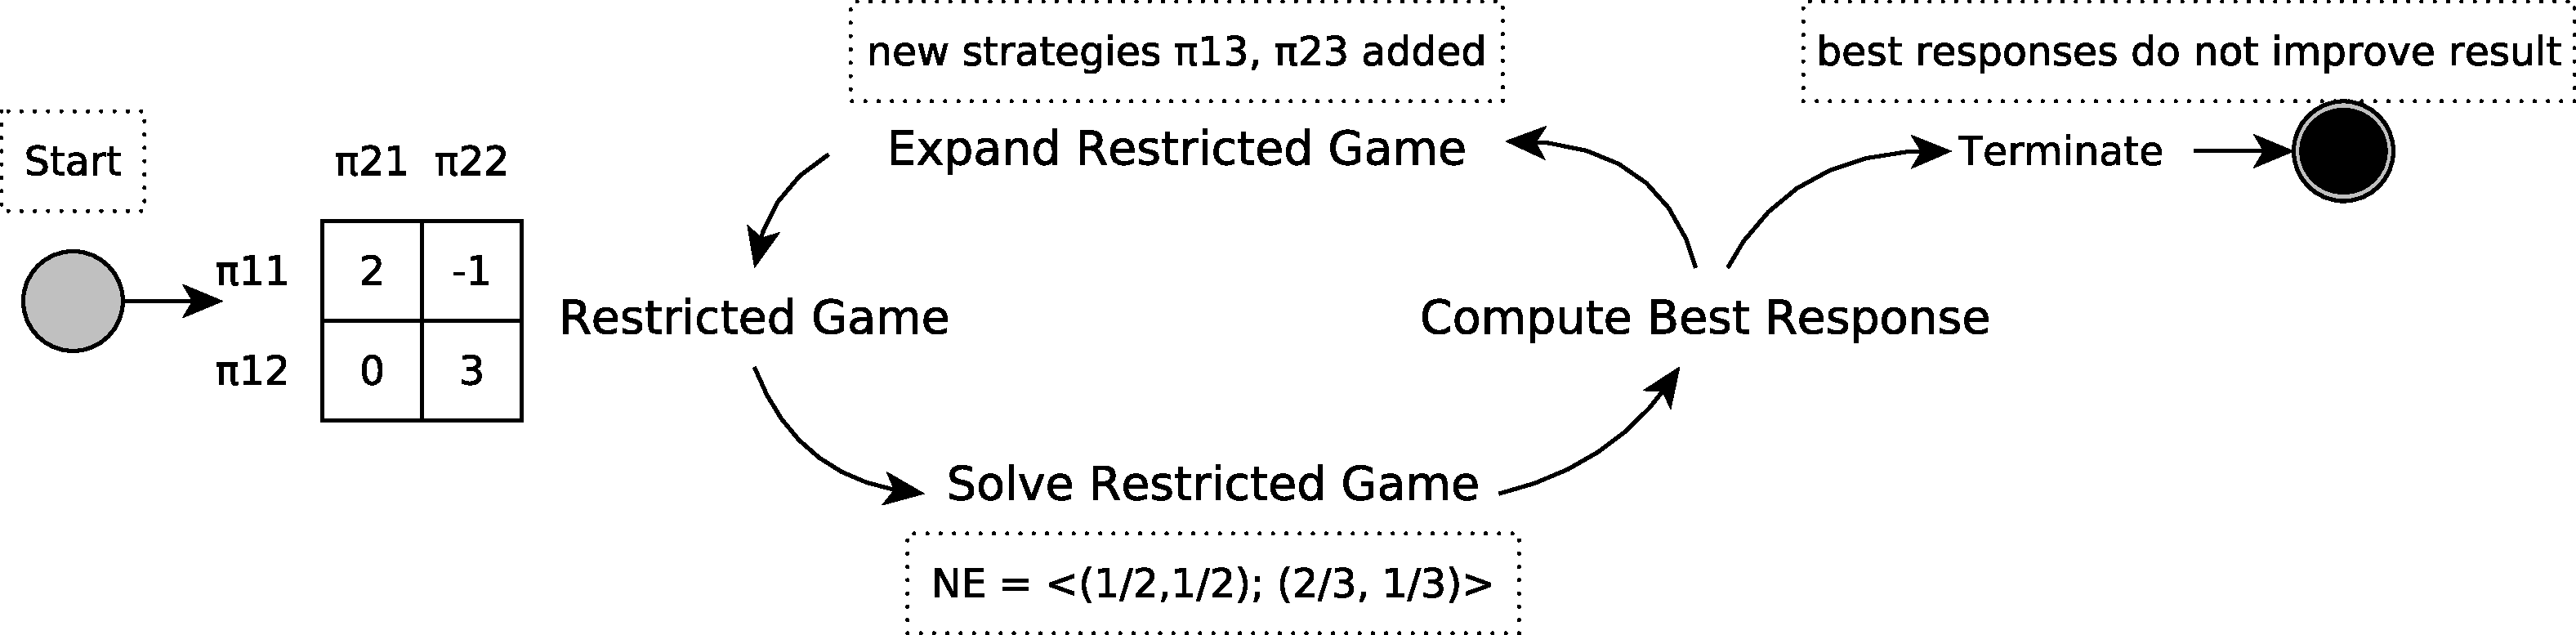
\includegraphics[width=0.8\textwidth]{figures/DO-scheme}
\caption{Schematic of the double-oracle algorithm for a normal-form game.}\label{fig:do-scheme}
\end{figure}

The main goal of the double-oracle algorithm is to find a solution of a matrix game without a need to construct the complete linear program that solves this game. 
The main idea is to create a restricted game by restricting the players to choose only from a limited set of actions.
Then the algorithm iteratively expands the restricted game by allowing the players to choose from new actions.
The new actions are allowed in iterations; each iteration a best response to an optimal strategy of the opponent in the current restricted game is allowed to be played in the restricted game.

Figure~\ref{fig:do-scheme} shows a visualization of the main structure of the algorithm, where the following three steps repeat until convergence:
\begin{enumerate}
\item create a restricted matrix game by limiting the set of actions that each player is allowed to play
\item compute a pair of Nash equilibrium strategies in this restricted game using linear programming
\item for each player, compute a pure best response strategy against the equilibrium strategy of the opponent; pure best response can be \emph{any} action from the original unrestricted game
\end{enumerate}
The best response strategies computed in step 3 are added to the restricted game, the game matrix is expanded by adding new rows and columns, and the algorithm follows with the next iteration. The algorithm terminates if neither of the players can improve the outcome of the game by adding a new strategy to the restricted game; hence, players play best response strategies to the strategy of the opponent. The algorithm maintains the values of expected utilities of the best-response strategies throughout the iterations of the algorithm. These values provide bounds on the value of the original game $v^*$

\subsubsection{Integrating Double-Oracle with Backward Induction}
\begin{algorithm2e}[t]
\small
\SetKwInOut{Input}{input}\SetKwInOut{Output}{output}
\Input{$s$ -- current matrix game; $i$ -- searching player; $\alpha_s,\beta_s$ -- bounds for the game value rooted in state $s$}
\If{$s \in \cZ$} {\Return $u_i(s)$} \label{alg:doab:stop1}
\If{$v_s^{-i} = v_s^i$} {
	\Return $v_s^{i}$
}
initialize $\cA'_i$, $\cA'_{-i}$ with arbitrary actions from $\cA_i, \cA_{-i}$\; \label{alg:doab:init}
\Repeat{$\alpha_s = \beta_s$}{
	\For{$r \in \cA'_i$, $c \in \cA'_{-i}$}{\label{alg:doab:restr1}
		\If{$A'_{rc}$ is not initialized}{
			 $A'_{rc} \leftarrow 0$\;
			\For{$s' \in S \;:\; \Delta_{\cT(s,r,c)}(s') > 0$} {
			$v^i_{s'} \leftarrow \textrm{alpha-beta}(s',i)$\; 
			$v^{-i}_{s'} \leftarrow \textrm{alpha-beta}(s',-i)$\; 
			\If{$v^{-i}_{s'} < v^i_{s'}$} {
				$A'_{rc} \leftarrow A'_{rc} + \Delta_{\cT(s,r,c)}(s')\cdot \textrm{double-oracle}(s',i,v^{-i}_{s'},v^i_{s'})$ \label{alg:doab:recursive}\;	
				}
			\Else{
				$A'_{rc} \leftarrow A'_{rc} + \Delta_{\cT(s,r,c)}(s')\cdot v^i_{s'}$ \label{alg:doab:saving}
				}
			}
		}	
	}
	$\left\langle v_s, \delta' \right\rangle \leftarrow $ solve matrix game $A'$\; \label{alg:doab:NE}
	$\left\langle v^{BR}_i, a^{BR}_{i} \right\rangle \leftarrow $ best-response$(i, \delta'_{-i}, \alpha_s)$\;\label{alg:doab:br1}
	$\left\langle v^{BR}_{-i}, a^{BR}_{-i} \right\rangle \leftarrow $ best-response$(-i, \delta'_{i}, \beta_s)$\; \label{alg:doab:br2}
	$\alpha_s \leftarrow \max(\alpha_s, v^{BR}_i)$,
	$\beta_s \leftarrow \min(\beta_s, v^{BR}_{-i})$\; \label{alg:doab:bounds}
	$\cA'_i \leftarrow \cA'_i \cup \lbrace a^{BR}_i \rbrace$,
	$\cA'_{-i} \leftarrow \cA'_{-i} \cup \lbrace a^{BR}_{-i} \rbrace$ \label{alg:doab:expand}
}
\Return $v_s$ \label{alg:doab:stop2}
\caption{Double Oracle with Serialized Bounds}\label{alg:doab}
\end{algorithm2e}

Double-oracle algorithm for matrix games can be directly incorporated into the backward induction -- instead of immediately evaluating each of the successors of the current game state and solving the linear program, the algorithm can exploit the double-oracle algorithm. Pseudocode in Algorithm~\ref{alg:doab} depicts this integration. In each state of the game, the algorithm initializes the restricted game with an arbitrary action (line~\ref{alg:doab:init}). Afterwards, the algorithm needs to evaluate each of the successors of the restricted game, for which the current value is not known (lines~\ref{alg:doab:restr1}-\ref{alg:doab:saving}). This evaluation is same as for backward induction with alpha-beta algorithm. 

Once all values for the restricted game $A'$ are known, the algorithm solves the restricted game (line~\ref{alg:doab:NE}) and keeps the optimal strategies $\delta'$ of the restricted game. Next, the algorithm calculates best responses for each of the player~(lines~\ref{alg:doab:br1},\ref{alg:doab:br2}), and updates the lower and upper bounds (line~\ref{alg:doab:bounds}). Finally, the algorithm expands the restricted game with best response actions (line~\ref{alg:doab:expand}) until the lower and upper bound are equal. In this case, neither of the best responses improves the current solution from the restricted game; hence, the algorithm has found an equilibrium of the complete unrestricted matrix game corresponding to state $s$.


\begin{algorithm2e}[t]
\small
\SetKwInOut{Input}{input}\SetKwInOut{Output}{output}
\Input{$s$ -- current matrix game; $i$ -- best-response player; $\lambda$ -- bound for the best-response value; $\delta'_{-i}$ -- strategy of the opponent }
$v^{BR}_i \leftarrow \lambda$ \;
$a_i^{BR} \leftarrow \textbf{null}$ \;
\For{$a_i \in \cA_i $\label{alg:br:start}} {%\setminus \cA'_i 
	$v_{a_i} \leftarrow 0$\;
	\For{$a_{-i} \in \cA'_{-i} \;:\; \delta'_{-i}(a_{-i}) > 0$} {\label{alg:br:opp}
		$\lambda_{a_i} \leftarrow \frac{v_i^{BR} - \sum_{a'_{-i} \in \cA'_{-i} \setminus \lbrace a_{-i} \rbrace} \delta'_{-i}(a'_{-i}) \cdot v^i_{\cT(s,a_i,a'_{-i})}}{\delta'_{-i}(a_{-i})}$\; \label{alg:br:bound}
		\If{	$\lambda_{a_i} > v^i_{\cT(s,a_i,a_{-i})}$}{
		continue from line~\ref{alg:br:start} with next $a_i$
		}
		\Else{
		\For{$s' \in S \;:\; \Delta_{\cT(s,a_i,a_{-i})}(s') > 0$} {
%			$v^i_{s'} \leftarrow \textrm{alpha-beta}(s',i)$\; \label{alg:br:ab1}
%			$v^{-i}_{s'} \leftarrow \textrm{alpha-beta}(s',-i)$\; \label{alg:br:ab2}
			\If{$v^{-i}_{s'} < v^i_{s'}$} {
				$v_{a_i,a_{-i}} \leftarrow v_{a_i,a_{-i}} + \Delta_{\cT(s,a_i,a_{-i})}(s')\cdot$ $\textrm{double-oracle}(s',i,v^{-i}_{s'},v^i_{s'})$\label{alg:br:recursive}\;	
				}
			\Else{
				$v_{a_i,a_{-i}} \leftarrow v_{a_i,a_{-i}} + \Delta_{\cT(s,a_i,a_{-i})}(s')\cdot v^i_{s'}$ \label{alg:br:saving}
				}
			}
			$v_{a_i} \leftarrow v_{a_i} + \delta'_{-i}(a_{-i})\cdot v_{a_i,a_{-i}}$\;		
		}
	}
	\If{$v_{a_i} > v_i^{BR}$}{\label{alg:br:max}
		$v_i^{BR} \leftarrow v_{a_i}$\;
		$a_i^{BR} \leftarrow a_i$\label{alg:br:save}
	} 
}
\Return $\langle v_i^{BR}, a_i^{BR} \rangle$ 
\caption{Best Response with Serialized Bounds}\label{alg:br}
\end{algorithm2e}

Next, we describe the algorithm for calculating the best responses. 
The pseudocode of the algorithm is depicted in Algorithm~\ref{alg:br}.
The goal of the algorithm is to find the best action from the original unrestricted game against current strategy of the opponent $\delta'$. 
Throughout the algorithm we use, as before, $v^i_{s'}$ to denote the upper bound of the value of the sub-game rooted in state $s'$ calculated using alpha-beta$(s',i)$. These values are calculated on demand, i.e., they are calculated once needed and cached until the game for state $s$ is not solved.
Moreover, once the algorithm calculates the exact value of a particular subgame, both upper and lower bounds are updated to be equal to actual value of the game. 

The algorithm iteratively tries all actions of player $i$ from the unrestricted game (line~\ref{alg:br:start}). 
Every action $a_i$ is evaluated against the actions of the opponent that are used in the optimal strategy from the restricted game (line~\ref{alg:br:opp}).
Before evaluating against an action of the opponent the algorithm determines, whether the current action of the searching player, $a_i$, can still be the best response action (line~\ref{alg:br:bound}). 
The value $\lambda_{a_i}$ represents the lowest possible expected utility this action must gain against the current action of the opponent $a_{-i}$. 
If this value is strictly higher than the upper bound of the successor (i.e., the value $v^i_{\cT(s,a_i,a_{-i})}$) than the algorithm knows that the action $a_i$ can never be the best response action, and the algorithm proceeds with the next action.
$\lambda_{a_i}$ is calculated by subtracting from the current best response value ($v_i^{BR}$) upper bound of the expected value against all other actions of the opponent ($v^i_{\cT(s,a_i,a'_{-i})}$). Recall, that these values are updated once the algorithm calculates exact values.

If the currently evaluated action $a_i$ can still be the best response, the value of the successor is determined (first by comparing the bounds). Once the expected outcome against all actions of the opponent is evaluated, the expected value of action $a_i$ is compared against the current best-response value (line~\ref{alg:br:max}) and saved, if the expected utility is higher~(line~\ref{alg:br:save}).


\subsection{Simultaneous-Move Monte Carlo Tree Search (SM-MCTS)}\label{sec:smmcts}

Monte Carlo Tree Search (MCTS) is a simulation-based state space search algorithm often used
in game trees. The nodes in the tree represent game states. The main idea is to iteratively run
simulations to a terminal state, incrementally growing a tree rooted at the initial state of the game. In
its simplest form, the tree is initially empty and a single leaf is added each iteration. Each iteration
starts by visiting nodes in the tree, selecting which actions to take based on a selection function and
information maintained in the node. Consequently, the algorithm transitions to a successor state. When a
node is visited whose immediate children are not all in the tree, the node is expanded by adding a
new leaf to the tree. Then, \emph{a rollout policy} (e.g., random action selection) is applied from the new
leaf to a terminal state. The outcome of the simulation is then returned as a reward to the new leaf
and the information stored in the tree is updated.

\begin{algorithm2e}[t]
\small
\SetKwInOut{Input}{input}\SetKwInOut{Output}{output}
\Input{$s$ -- current state of the game; $i$ -- current player}
\If{$s \in \cZ$} {
	\Return \emph{\underline{RetValLeaf}}($u_i(s)$)
}
\If{$s \in T$} {
	$(a_i, a_{-i}) \leftarrow$ \emph{\underline{Select}}$(s)$\;\label{alg:smmcts:select}
	$s' \leftarrow \cT(s,a_i,a_{-i})$\;
	$v_{s'} \leftarrow $ SM-MCTS($s',i$)\;
	$v_{s} \leftarrow$ \emph{\underline{Update}}$(s,a_i,a_{-i},v_{s'})$\;\label{alg:smmcts:up}
	\Return $v_{s}$
}
\Else{
	$T \leftarrow T \cup \lbrace s \rbrace$\;
	$v_{s} \leftarrow $ \emph{\underline{Rollout}}($s$)\;
	\Return $v_{s}$
}

%\If{$s \in T \wedge \exists(a_i, a_{-i}) \in \cA(s)$~not previously visited} {
%	choose one of the previously unselected $(a_i, a_{-i})$\;
%	$s' \leftarrow \cT(s,a_i,a_{-i})$\;
%	$T \leftarrow T \cup \lbrace s' \rbrace$\;
%	$v_{s'} \leftarrow $ \emph{\underline{Rollout}}($s'$)\;
%	$X_{s'} \leftarrow X_{s'} + v_{s'}$\;
%	$n_{s'} \leftarrow n_{s'} + 1$\;
%	\emph{\underline{Update}}$(s,a_i,a_{-i},v_{s'})$\;\label{alg:smmcts:up1}
%	\Return \emph{\underline{RetVal}}$(v_{s'}, X_{s'}, n_{s'})$ 	
%}
%\Else{
%	$(a_i, a_{-i}) \leftarrow$ \emph{\underline{Select}}$(s)$\;\label{alg:smmcts:select}
%	$s' \leftarrow \cT(s,a_i,a_{-i})$\;
%	$v_{s'} \leftarrow $ SM-MCTS($s',i$)\;
%	$X_{s} \leftarrow X_{s} + v_{s'}$\;
%	$n_{s} \leftarrow n_{s} + 1$\;
%	\emph{\underline{Update}}$(s,a_i,a_{-i},v_{s'})$\;\label{alg:smmcts:up2}
%	\Return \emph{\underline{RetVal}}$(v_{s'}, X_{s}, n_{s})$ 	
%}
\caption{Simultaneous Move Monte Carlo Tree Search}\label{alg:smmmcts}
\end{algorithm2e}

We first present a generic template of MCTS algorithms for simultaneous move games (SM-MCTS) and then explain specific algorithms derived form this template. Algorithm~\ref{alg:smmmcts} describes a single iteration of the SM-MCTS. $T$ represents the MCTS tree, in which
each state is represented by one node. Every node $s$ maintains algorithm-specific statistics about the iterations that previously used this node. The template can be instanciated by specific implementations of the updates of the statistics on line~\ref{alg:smmcts:up} and the selection based on these statistics on line \ref{alg:smmcts:select}. 
Different algorithms can be the bases for the selection functions (e.g., UCB~\cite{UCB}, Exp3~\cite{Auer2003Exp3}, regret matching~\cite{Hart00}, or CFR~\cite{}) and we describe them in the following sections. 
Moreover, different selection functions need different statistics kept in each node; hence, function \emph{\underline{Update}} also differs. 
Finally, some algorthms require collecting statistics form more then just the current node during the iteration.
These statistics are returned be the main iteration function, they can be initialized in \emph{\underline{RetValLeaf}} and further updated as a part of the \emph{\underline{Update}} function.
For the most basic SM-MCTS algorithms, only the curent sample value is returned by the function and none of these functions modifies it.

\subsubsection{Decoupled Upper-confidence Bound applied to Trees}

The most common selection function for SM-MCTS is the Decoupled Upper-confidence Bound applied to Trees(DUCT). For selection and updates, it executes the well-known UCT \cite{kocsis2006} algorithm independently for each of the players in each nodes. The statistics stored in search nodes are independently computed for each action of each player. For player $i\in N$ and action $a_i \in A_i(s)$ the reward sums $X_{a_i}$ and the number of times the action was used $n_{a_i}$ are maintained. When a joint action needs to be selected on line 
\ref{alg:select}, an action that maximizes the UCB value over their reward estimates is selected for each player independently:
\[ a_i = \argmax_{a \in A_i(s)}{ \left\{ \bar{X}_{a_i} + C_i \sqrt{\frac{\log n_s}{n_{a_i}}} \right\} }, 
  \mbox{ where } \bar{X}_{a_i} = \frac{X_{a_i}}{n_{a_i}} \mbox{ and } n_s=\sum_{a_j} n_{a_j}. \] 
\noindent The update policy increases the visit count and rewards for each player $i$ using $X_{a_i} \leftarrow X_{a_i} + u_i$ 
and $n_{a_i} \leftarrow n_{a_i} + 1$. The \emph{\underline{RetValLeaf}} and  \emph{\underline{Rollout}} just return the value of the leaf node reach and  \emph{\underline{Update}} does not modify this value. The same value is back-propagated to the root of the MCTS tree.

After all the simulations are done, there are two options how to determine the resulting action to play. The more standard opttion is to choose for each state the joint move that maximizes $n_{a_i}$ for each player $i$ independently.
This is suitable mainly for games, in which using mixed strategy is often not necessary.
Alternatively, the action to play in each state can be determined based on the mixed strategy obtained by normalizing the visit counts of each action ($n_{a_i}$).
Using the first method will certainly not make the algorithm converge to a Nash equilibirum, because the game may require a mixed strategy.
The second has been shown not to converge to a Nash equilibrium as well; a counter-example in Rock, Paper, Scissors with biased payoffs is shown in \cite{Shafei09}. 

Even though DUCT is not guaranteed to converge to the optimal solution, it is often very successful in practice.
It has been used in and general game playing~\cite{Finnsson12}, in the Internet card game Urban Rivals~\cite{Teytaud11Upper},
and in the simultaneous move game Tron~\cite{Perick12Comparison}. 
\mlanctot{Is there an earlier Tron paper where it was used?}
Note that DUCT is different than UCT run on a game that is transformed to perfect information by serialization of the simultaneous moves, 
because in the latter case one player has the advantage of knowing what the other player chose at every stage.


\subsubsection{Decoupled Exponential weights for Exploration and Exploitation}\label{sec:exp3}

The second most common instantiation of SM-MCTS is to use the Exponential weights for Exploration and Exploitation (Exp3) algorithm \cite{Auer2003Exp3} independently for each of the players. In Exp3, a player maintains an estimate of the sum of rewards for each action, denoted $\hat{X}_{a_i}$. The joint action selected on line \ref{alg:select} is composed of an action independently selected for each player. The probability of sampling action $a_i$ in \emph{\underline{Select}} is proportional to the exponential of the reward estimate:
\begin{equation}\label{eq:exp3select}
\sigma^s(a_i) = \frac{(1-\gamma) \exp(\eta \hat{X}_{a_i})}{\sum_{b_i \in A_i(s)} \exp(\eta \hat{X}_{a_i})} + \frac{\gamma}{|A_i(s)|},
  \mbox{ where } \eta = \frac{\gamma}{|A_i(h)|}.
\end{equation}

This standard formulation of Exp3 is suitable for proving its properties, but straightforward implementation of this formula leads to problems with numerical stability. Both the numerator and denominator of the fraction are too large. For this reason, numerically more stable formulations has been suggested, e.g., in \cite{Lanctot13Goofspiel} and \cite{Cowling12ISMCTS}. We use the following reformulation from \cite{Cowling12ISMCTS}:
\begin{equation}
\sigma^s(a_i) = \frac{(1-\gamma)}{\sum_{b_i \in A_i(s)}\exp(\eta(\hat{X}_{b_i}-\hat{X}_{a_i}))}
\end{equation}


The \underline{Update} after selecting actions $(i,j)$ and obtaining a result $(u_1,u_2)$ updates the visits count ($n_{h,i} \leftarrow n_{h,i} + 1$) and adds to the corresponding reward sum estimates the reward divided by the probability that the action was played by the player ($x_{h,i} \leftarrow x_{h,i} + u_1/\sigma^s(h,i)$). 
%The rewards are assumed to be normalized to the unit interval. 
Dividing the value by the probability of selecting the corresponding action makes $x_{h,i}$ estimate the sum of rewards over all iterations, not only the once where action $i$ was selected. 
%We are using a numerically more stable version of the formula for computing the distribution presented in \cite{Cowling12ISMCTS}, which is equivalent to the original one \cite{Auer2003Exp3}.

%The mixed (\ie randomized) strategy used by player $i$ after the simulations are done is given by the frequencies of visit counts of the actions: $\sigma^{final}(h,i) = n_{h,i}/\sum_{i' \in A_i(h)} n_{h,i'}$. Previous work \cite{Teytaud11Upper} suggests first removing the samples caused by the exploration. This modification proved to be useful also in our experiments, so before computing the resulting final mixed strategy, we set
%\begin{equation}
%n_{h,i} \leftarrow \max\left(0,n_{h,i} - \frac{\gamma}{|A_i(h)|}\sum_{i' \in A_i(h)}n_{h,i'}\right).
%\end{equation}


\subsubsection{Regret Matching}

\subsubsection{Online Counter-factual Regret Minimization}

